\documentclass[tikz, border=10pt]{standalone}
\usepackage[dvipsnames]{xcolor}
\usepackage{pgfplots}
\pgfplotsset{compat=1.18}
\usetikzlibrary{calc,positioning,arrows.meta}

\tikzset{
  black arrow/.style={-stealth, thick},
  node box/.style={draw=black, fill=white, text=black, rectangle, rounded corners, font=\small, align=center, minimum height=2em},
  % FIXED: Manual path for stability. No sin/cos calculations to crash the engine.
  eeg wave/.pic={
    \draw[purple, thick, x=0.05cm, y=0.15cm] 
      (0,0) -- (1,1) -- (2,-1) -- (3,1.5) -- (4,-1.2) -- (5,0.8) -- 
      (6,-0.5) -- (7,1.2) -- (8,-1.5) -- (9,0.5) -- (10,0);
  }
}

\begin{document}
\begin{tikzpicture}[font=\sffamily]

  % --- ROOT DATA INPUT ---
  \node[node box, fill=blue!20] (root) {5-second Epoch Data};

  % --- EEG BRANCH ---
  \node[node box, below left=1cm and 0cm of root] (eeg_input) {
    EEG Signal Data \tikz[baseline=-0.5ex]{\pic {eeg wave}}
  };
  % \node[right=0.2cm of eeg_input] (wave_pos) {}; 
  % \path (wave_pos) pic {eeg wave};
  
  \node[node box, below=1cm of eeg_input] (eeg_bagging) {EEG Feature Bagging};
  
  % EEG Forest Representative Trees (placed as images)
  \node[inner sep=0pt] at ($(eeg_bagging)+(-1.5cm,-2.5cm)$) (et1) {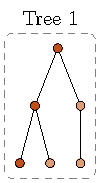
\includegraphics{eeg_tree1}};
  \node[inner sep=0pt] at ($(eeg_bagging)+(1.5cm,-2.5cm)$) (etn) {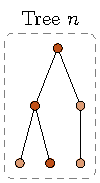
\includegraphics{eeg_treen}};

  \node[node box, below=4.5cm of eeg_bagging] (eeg_avg) {Averaging};
  \node[node box, fill=Salmon!50, below=1cm of eeg_avg] (eeg_pred) {EEG Prediction:\\(Awake, N1, N2, N3, REM)};

  % --- IMU BRANCH ---
  \node[node box, below right=1cm and 0cm of root] (imu_input) {IMU Signal Data \textbf{\textit{a}}};
  \node[node box, below=1cm of imu_input] (imu_bagging) {IMU Feature Bagging};

  \node[inner sep=0pt] at ($(imu_bagging)+(-1.5cm,-2.5cm)$) (it1) {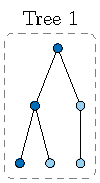
\includegraphics{imu_tree1}};
  \node[inner sep=0pt] at ($(imu_bagging)+(1.5cm,-2.5cm)$) (itn) {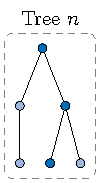
\includegraphics{imu_treen}};

  \node[node box, below=4.5cm of imu_bagging] (imu_avg) {Averaging};
  \node[node box, fill=BurntOrange!50, below=1cm of imu_avg] (imu_pred) {IMU Prediction:\\(Awake vs. Asleep)};

  % --- OVERRIDE LOGIC ---
  \node[node box, fill=Goldenrod!50, below=1cm of eeg_pred.south, minimum width=4cm] (logic) {
    Override Logic:\\
    \textbf{IF} EEG = N1 \textbf{AND} IMU = Awake\\
    \textbf{THEN} Final = Awake
  };

  \node[node box, fill=SpringGreen, below=1cm of logic, minimum width=5cm, font=\bfseries] (final) {Final Sleep Stage Output};

  % --- CONNECTIONS ---
  \draw[black arrow] (root) -- (eeg_input);
  \draw[black arrow] (root) -- (imu_input);
  
  \draw[black arrow] (eeg_input) -- (eeg_bagging);
  \draw[black arrow] (eeg_bagging) -- (et1);
  \draw[black arrow] (eeg_bagging) -- (etn);
  \draw[black arrow] (et1) -- (eeg_avg);
  \draw[black arrow] (etn) -- (eeg_avg);
  \draw[black arrow] (eeg_avg) -- (eeg_pred);

  \draw[black arrow] (imu_input) -- (imu_bagging);
  \draw[black arrow] (imu_bagging) -- (it1);
  \draw[black arrow] (imu_bagging) -- (itn);
  \draw[black arrow] (it1) -- (imu_avg);
  \draw[black arrow] (itn) -- (imu_avg);
  \draw[black arrow] (imu_avg) -- (imu_pred);

  \draw[black arrow] (eeg_pred) -- (logic);
  \draw[black arrow] (imu_pred) |- (logic);
  \draw[black arrow] (logic) -- (final);

  % Ellipsis for forests
  \path (et1) -- (etn) node [midway, scale=2] {$\dots$};
  \path (it1) -- (itn) node [midway, scale=2] {$\dots$};

\end{tikzpicture}
\end{document}